\section{Introduction}
Compartmental models have become important tools for investigating
the behaviour of neurons to the extent that a number of packages
exist to facilitate their implementation (\emph{e.g.} Hines and
Carnevale \cite{Hines97}; Bower and Beeman \cite{Bower97}). The
use of compartmental models is motivated by the desire to reduce
the mathematical complexity inherent in a continuum description of
a neuron. This simplification is achieved by replacing the family
of partial differential equations defining the continuum
description of a neuron by a compartmental model of that neuron in
which the behaviour of the neuron is described in terms of the
solution of a family of ordinary differential equations (Rall,
\cite{Rall64}). The traditional approach to compartmental
modelling, introduced by Rall (\cite{Rall64}), assumes that a
``lump of membrane becomes a compartment; the rate constants
governing exchange between compartments are proportional to the
series conductance between them". Figure \ref{Rall} illustrates
the Rall interpretation of a how a dendrite can be represented in
terms of compartments (neuronal membrane) and linking resistances
(the axoplasm).

\begin{figure}[!h]
\centering
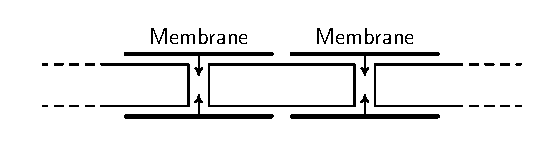
\includegraphics[ ]{NewCompFig1.eps}
\parbox{5in}{\caption{\label{Rall}
The Rall segmentation of a length of dendrite into lumped regions.
The membrane defines the compartment, and the resistive property
of the axoplasm is represented in the model by resistors linking
compartments}}
\end{figure}

%\begin{figure}[!h]
%\centerline{\begin{mfpic}[1][1]{0}{250}{-25}{35}
%\pen{1pt}
%\lines{(30,10),(70,10),(70,-10),(30,-10)}
%\dashed\lines{(30,10),(0,10)}
%\dashed\lines{(30,-10),(0,-10)}
%\rect{(80,10),(150,-10)}
%\lines{(200,10),(160,10),(160,-10),(200,-10)}
%\dashed\lines{(200,10),(230,10)}
%\dashed\lines{(200,-10),(230,-10)}
%\arrow\lines{(75,15),(75,5)}
%\arrow\lines{(75,-15),(75,-5)}
%\arrow\lines{(155,15),(155,5)}
%\arrow\lines{(155,-15),(155,-5)}
%\pen{2pt}
%\headlen7pt
%\lines{(40,15),(110,15)}
%\lines{(40,-15),(110,-15)}
%\lines{(120,15),(190,15)}
%\lines{(120,-15),(190,-15)}
%\tlabel[bc](75,20){\textsf{Membrane}}
%\tlabel[bc](155,20){\textsf{Membrane}}
%\end{mfpic}}
%\centering
%\parbox{5in}{\caption{\label{Rall}
%The Rall segmentation of a length of dendrite into lumped regions.
%The membrane defines the compartment, and the resistive
%property of the axoplasm is represented in the model by resistors
%linking compartments}}
%\end{figure}

This partitioning of a dendrite into repeating units is analogous
to the representation of a transmission line as a ladder network
of simple electrical circuits. In the case of a neuron, Rall
defines a compartment to be the mathematical description of the
effect of input acting on a localised region of neuronal membrane,
and models this by an electrical circuit. The resistive properties
of the axoplasm determine the linking resistances between
compartments. Other authors (\emph{e.g.} Segev and Burke,
\cite{Segev98}) treat the neuronal segment, including the membrane
and axoplasm, as the compartment. However both definitions lead to
the same mathematical model simply because the iso-potential
property, implicit in Rall (\cite{Rall64}) and explicit in Segev
and Burke's (\cite{Segev98}) definition of a compartment,
dominates the construction of the underlying family of ordinary
differential equations. However, the definition of a compartment
as an iso-potential region is unsatisfactory since a compartment
defined in this way cannot act as a fundamental unit in the
construction of a model dendrite for two good reasons. First,
iso-potential compartments must exist in pairs to support axial
current flow, and second, half compartments are required to
represent branch points and dendritic terminals (\emph{e.g.} Segev
and Burke, \cite{Segev98}).

What is required is a definition of a compartment in which the
compartment exists as an independent unit that can act as a
building block for a model of the electrical behaviour of a
neuron, where it is understood that ``the function of the model is
to represent the necessity that exists in nature by the logical
necessity of the model. In the case of a good model one parallels
the other'' (Regnier, \cite{Regnier64}).  A traditional
compartmental model does not satisfy this criterion since its
iso-potential structure provides no mechanism to differentiate
between input \emph{at different locations within the segment}
represented by the compartment. It is precisely through the
definition of a compartment, which allows this distinction to be
made, that the new compartment model gives superior accuracy and
precision to that of a traditional model.

The accuracy with which a compartmental model describes the
behaviour of a neuron may be assessed from the knowledge that all
compartmental models converge to the solution of the continuum
model of that neuron as the maximum length of segment approaches
zero. To take advantage of this result, a test neuron is
constructed for which the continuum description has an exact
solution. This test neuron and its exact solution are used as a
reference against which the accuracy of a traditional
compartmental model and the new compartmental model are compared.

\section{Structure of compartmental models}
We are concerned with compartmental models of dendrites. In this
context, the fundamental morphological unit is the dendritic
\emph{section}, defined to be the length of dendrite connecting
one branch point to a neighbouring branch point, to the soma or to
a terminal. Compartmental modelling begins by subdividing each
section of a dendrite into smaller contiguous units called
segments which are typically regarded as uniform circular
cylinders (\emph{e.g.} Segev and Burke, \cite{Segev98}) or tapered
circular cylinders (Hines and Carnevale \cite{Hines97}). The
mathematical model of a dendrite is constructed by representing
each segment by a compartment, and connecting these in a branching
pattern corresponding to that of the dendrite. When joined in this
way, each compartment interacts only with compartments
representing adjacent segments. Note that some numerical schemes
for the solution of the continuum model (\emph{e.g.}, Finite
Differences) may have this ``nearest neighbour'' property, but it
would be a conceptual error to interpret such equations as a
compartmental model. The ``nearest neighbour'' feature of these
equations is a contingent property of the numerical
algorithm\footnote{For example, a second order central difference
approximation for the spatial derivatives of the continuum model
will be structurally identical to a compartmental model when the
error structure of the discretisation is ignored. However, the
``nearest neighbour'' property of the numerical algorithm is
absent for a higher order finite difference scheme.} and vanishes
with a different choice of algorithm, whereas the ``nearest
neighbour'' feature of a compartmental model is unavoidable.

In a traditional compartmental model, the compartment has a single
potential which is viewed as the potential at the centre of the
segment represented by that compartment. This potential may be
thought of as the average potential of that segment. All
voltage-regulated input to the segment, independent of its
location, acts with this potential. The assumption that all input
to a segment acts with a single potential irrespective of location
on the segment implies that a traditional compartmental model
regards dendritic segments as iso-potential regions of dendrite.
Spatial variations in biophysical properties of the dendrite and
its morphology are expressed through differences in the properties
of compartments and their linking resistors.

By contrast, the new compartmental model assigns two potentials to
a compartment, one at each boundary of the segment represented by
the compartment. Compartments constructed in this way can serve as
the basic building blocks of a model dendrite because they sustain
axial currents independent of neighbouring compartments. Most
importantly, the assumption that transmembrane current acts at the
centre of a segment, as in a traditional compartmental model, is
now inappropriate and must be replaced in the new compartmental
model by a rule to partition transmembrane current between the
axial currents flowing at segment boundaries. As with the
traditional compartmental model, compartments in the new model are
connected together by enforcing conservation of axial current at
segment boundaries, dendritic branch points and dendritic
terminals.
